% !TEX program = lualatex
% !TEX recipe = latexmk (lualatex)
\documentclass{sice-si}

\def\LuaLaTeX{Lua\LaTeX}
\def\upLaTeX{up\LaTeX}
\def\pTeX{p\TeX}
\def\SICEcls{sice.cls}

\newcommand{\TeXEngine}{unknown}
\ifluatex
    \renewcommand{\TeXEngine}{\LuaLaTeX}
\else
    \ifuptex
        \renewcommand{\TeXEngine}{\upLaTeX}
    \fi
\fi

\usepackage{cite}

% Compact bibliography formatting
\let\oldthebibliography\thebibliography
\let\endoldthebibliography\endthebibliography
\renewenvironment{thebibliography}[1]{%
    \begin{oldthebibliography}{#1}%
        \fontsize{8.5pt}{10.5pt}\selectfont
        \setlength{\itemsep}{1.5pt}%
        \setlength{\parskip}{0pt}%
}{%
    \end{oldthebibliography}%
}

% タイトルと著者名
\title{シミュレーション環境における生成的群衆行動のための蒸留ビヘイビアツリーに基づくモデリング} % 和文タイトル
\name{○NGUYEN TRI TUNG NGUYEN（計測自動制御学会），細田侑也（計測自動制御学会），李俊浩（計測自動制御学会）} % 著者名
\etitle{Distilled Behavior Tree-Based Modeling For Generative Crowd Behavior in Simulation Environment.} % 英文タイトル
\ename{○NGUYEN TRI TUNG NGUYEN (SICE), HOSODA YUYA (SICE), and LEE JOO-HO}	%著者名（英）

\begin{document}
% アブストラクト
\abst{
    Although modern generative crowd architectures offer broad and high-quality behavioral coverage, their substantial runtime computational overhead impedes closed-loop deployment. To address this, we propose a novel behavior-tree-based generative framework that distills neural policies into explainable, deterministic structures suitable for open-loop robotic simulations.
}

% タイトルの出力
\maketitle

% 本文
\section{Introduction}
Simulating realistic multi-agent crowd behaviors is essential for evaluating autonomous vehicles and service robots in urban settings. Classical microscopic pedestrian models, such as the Social Force Model~\cite{helbing1995social} and Optimal Reciprocal Collision Avoidance (ORCA)~\cite{vandenberg2011reciprocal}, rely on explicit physical and geometric heuristics. While computationally efficient, they produce rigid, uniform maneuvers that struggle to capture the behavioral diversity, subtle concessions, and multimodality of real crowds.
\begin{figure*}[t]
    % First photo
    \centering
    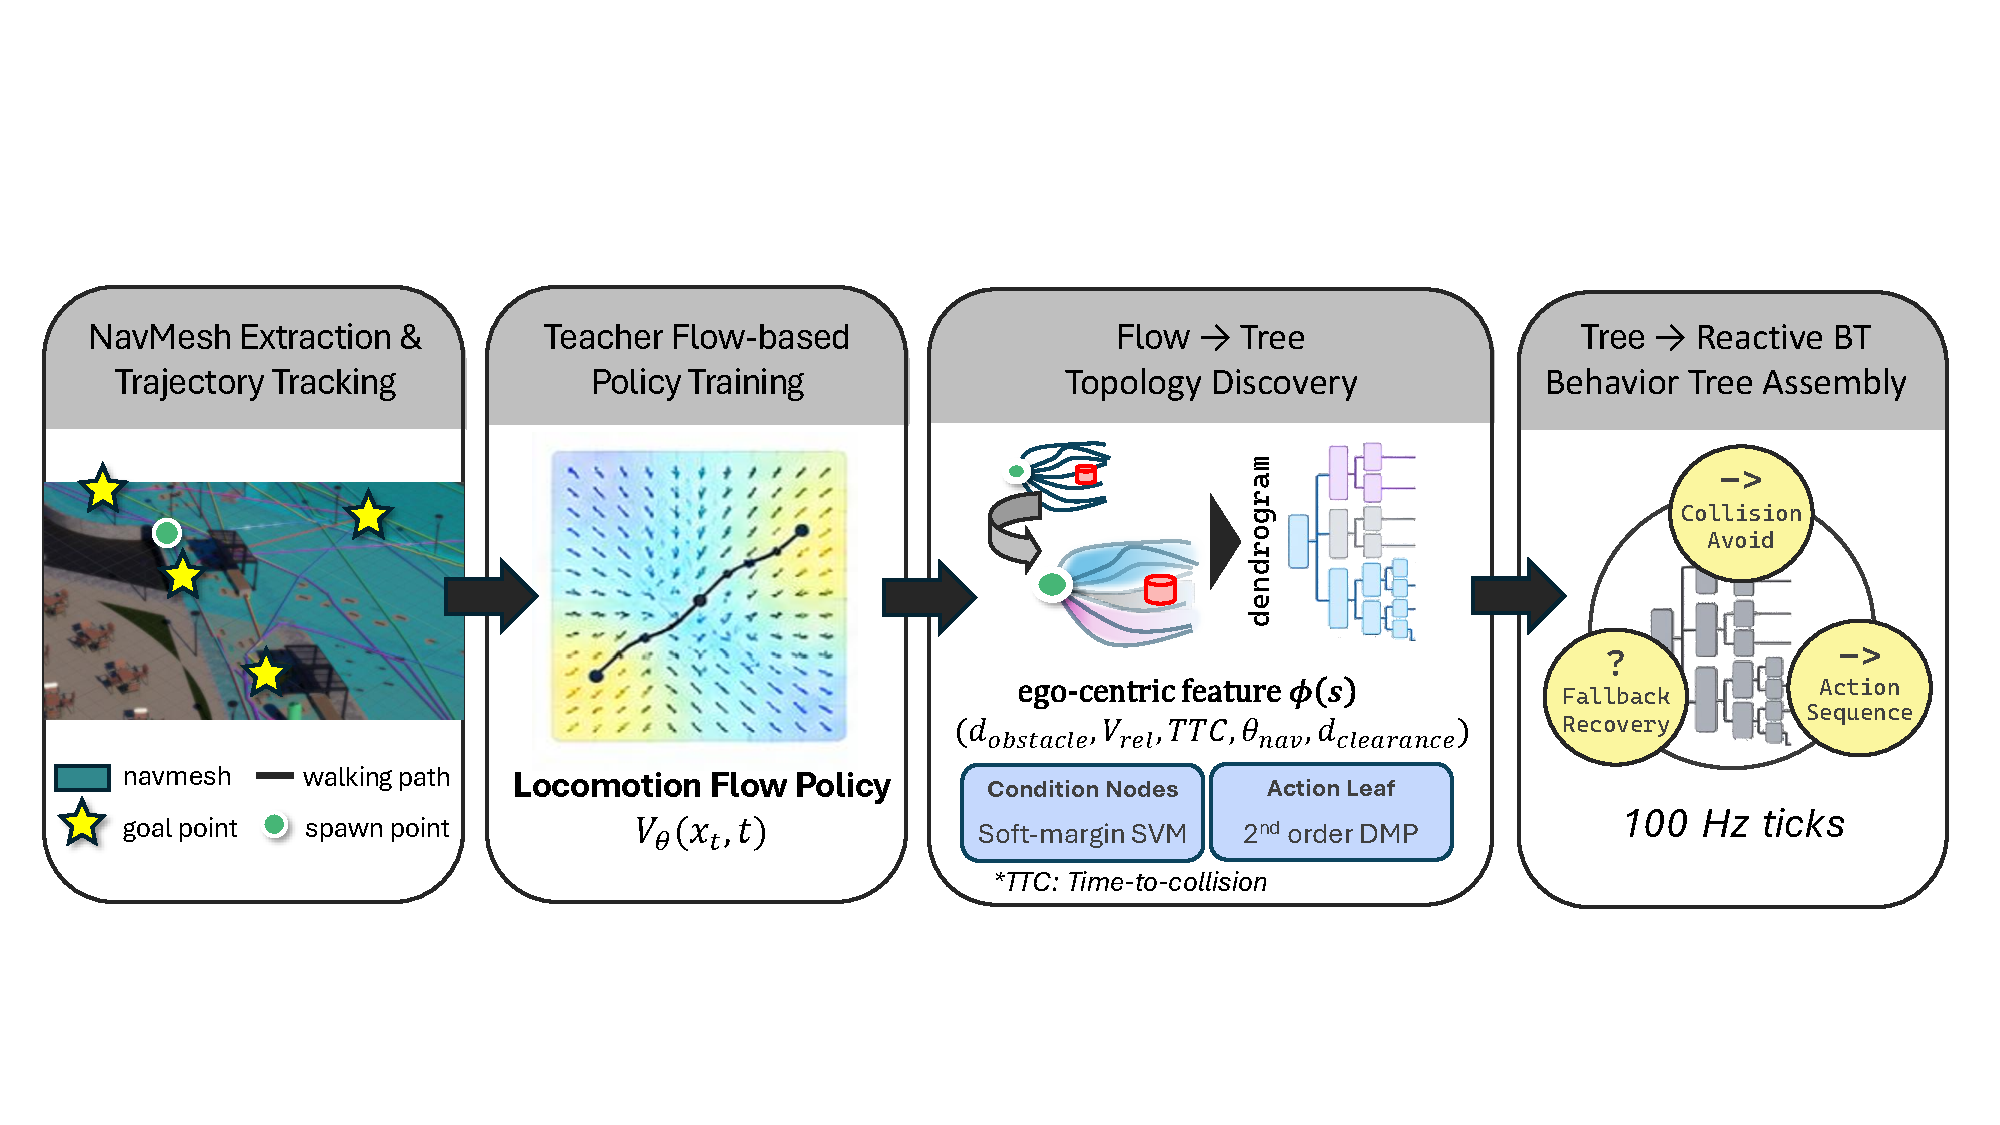
\includegraphics[width=0.95\textwidth,trim={0.6cm 3.5cm 0.8cm 3.5cm},clip]{figures/overview.pdf}
    \caption{
         Overview of the proposed Flow2BT framework. The generative flow matching model is used as a teacher to distill continuous multimodal pedestrian behaviors into a reactive, interpretable Behavior Tree (BT) with closed-form Dynamical Movement Primitive (DMP) leaves.
    }
    \label{fig:overview}
\end{figure*}

Recent approaches turn to deep generative modeling, such as continuous Flow Matching~\cite{lipman2023flow} in CrowdES~\cite{bae2025crowdes}, learning continuous velocity fields from demonstration data (e.g., ETH/UCY datasets). Despite their expressiveness, deploying deep generative models directly in closed-loop interactive simulations reveals two key structural limitations:
\begin{enumerate}[label=\arabic*), labelsep=0.5em, noitemsep, topsep=2pt]
    \item \textbf{Chunked Decision Latency:} Simulators generate paths in open-loop temporal chunks ($T_f = 2\,\text{s}$ at $5\,\text{fps}$) governed by modes predicted once per chunk. An agent trapped in this window cannot react to sudden intrusions, yielding a collision rate ($C_R \approx 0.78\%$) nearly two orders of magnitude higher than real human crowds ($C_R \approx 0.01\%$).
    \item \textbf{Black-Box Opacity:} End-to-end neural decoders map latent states directly into future coordinates without symbolic logic, preventing developers from auditing why an agent chose to yield, swerve, or stop.
\end{enumerate}

To resolve decision latency and black-box opacity while preserving generative realism, we propose \textbf{Flow2BT}, a framework that distills continuous generative crowd policies into interpretable \textit{Behavior Trees} (BT)~\cite{colledanchise2018behavior} paired with a decentralized CBF safety filter. Motivated by tree-flow duality~\cite{ramachandran2026trees}, our architecture treats the generative flow model as an expressive macro-teacher: we extract topological bifurcations in a NavMesh-aligned frame, induce linear condition hyperplanes, and compress unimodal branches into 2nd-order Dynamical Movement Primitives (DMPs)~\cite{chatzilygeroudis2021behavior}. Ticking at $100\,\text{Hz}$, the tree enables $10\,\text{ms}$ reactive preemption via Fallback control nodes upon sudden hazard detection.

Our key contributions and findings are as follows:
\begin{itemize}[noitemsep, topsep=2pt]
    \item \textbf{Neuro-Symbolic Distillation:} We show that continuous crowd policies can be distilled into interpretable Behavior Trees with closed-form DMP leaves, slashing reactive decision latency from $2000\,\text{ms}$ down to $10\,\text{ms}$.
    \item \textbf{Collision Mechanics Analysis:} We demonstrate that CBF filtering achieves exact forward invariance ($C_R = 0.0\%$) on raw states and empirically isolate post-processing mesh snapping as the primary source of reported collisions.
    \item \textbf{Certified Safety \& Realism:} Our synthesized BT + CBF controller achieves a \textbf{$3.1\times$ collision reduction} over state-of-the-art CrowdES ($0.00249$ vs. $0.00781$) while matching or improving travel time and population flow on standard benchmarks.
\end{itemize}

\section{Related Work}
\subsection{Generative Pedestrian Locomotion}
Simulating pedestrian dynamics has evolved from rule-based microscopic frameworks to high-capacity data-driven generative policies. Classical models such as the Social Force Model (SFM)~\cite{helbing1995social} and Optimal Reciprocal Collision Avoidance (ORCA)~\cite{vandenberg2011reciprocal} characterize agent interactions using repulsive potential fields and velocity-obstacle geometric cones. While computationally lightweight and mathematically tractable, these explicit physics heuristics struggle to capture the rich behavioral heterogeneity, subtle group interactions, and contextual multimodality observed in real human crowds, frequently suffering from unnatural oscillations or the ``freezing robot'' problem in dense bottleneck scenarios.

To overcome these constraints, recent approaches have embraced deep neural architectures, ranging from recurrent trajectory forecasters~\cite{alahi2016social} to Flow Matching~\cite{lipman2023flow}. In particular, CrowdES~\cite{bae2025crowdes} represents the state of the art in continuous crowd locomotive simulation, generating expressive multi-agent trajectories conditioned on NavMesh global waypoints. However, existing generative crowd simulators operate in an open-loop temporal chunking paradigm ($T_f = 2\,\text{s}$ at $5\,\text{fps}$), sampling discrete behavioral modes ($B=8$) only once per chunk. In dense interactive environments, an agent committed to an open-loop horizon cannot react to dynamic intrusions or sudden trajectory deviations of neighboring walkers, leading to elevated collision rates that diverge from real human crowds.

\subsection{Behavior Trees and Robot Control}
Behavior Trees (BTs) have emerged as a premier architectural paradigm for modular and reactive robot control~\cite{colledanchise2018behavior,iovino2022survey}. By recursively organizing execution logic into Sequence ($\to$) and Fallback ($?$) control nodes, BTs achieve instantaneous task preemption, transparent precondition auditing, and formal composability. Despite these advantages, synthesizing BT structures from demonstration data remains a formidable challenge. Classical search methods such as Genetic Programming (GP-BT)~\cite{iovino2022survey} suffer from combinatorial explosion and tree bloat, requiring hundreds of thousands of candidate evaluations. Conversely, continuous differentiable relaxations~\cite{huang2025differentiable} often exhibit a severe discretization-execution gap when softened routing probabilities are hardened for discrete deployment.

To bridge continuous motion and symbolic execution, trajectory-based BTs and Dynamical Movement Primitives (DMPs)~\cite{chatzilygeroudis2021behavior,ijspeert2013dynamical} encapsulate motor skills within parameterized attractor systems. Recently, Ramachandran and Sra~\cite{ramachandran2026trees} established a rigorous mathematical duality between continuous flows and hierarchical trees: under reverse-time coarse-graining, continuous velocity fields naturally coalesce into discrete hierarchical dendrograms. Flow2BT builds on this foundational insight, treating continuous flow policies as macro-teachers to induce interpretable BT topologies without heuristic grammar search.

\section{Proposed Method}
As illustrated in \Fig{fig:overview}, the proposed Flow2BT architecture systematically distills a high-capacity continuous generative crowd policy into a certified, reactive Behavior Tree. The pipeline is structured into three interconnected operational stages:
\begin{enumerate}[label=\arabic*), labelsep=0.5em]
    \item \textbf{Teacher Flow-Based Policy Training:} Learning continuous locomotive vector fields conditioned on global NavMesh tracking and ego-centric multi-agent context.
    \item \textbf{Flow-to-Tree Topology Discovery:} Rolling out continuous trajectory ensembles and extracting a hierarchical decision dendrogram via reverse-time coarse-graining.
    \item \textbf{Tree-to-Reactive BT Assembly:} Inducing maximum-margin condition guards, parameterizing action leaves into 2nd-order DMPs, and assembling a $100\,\text{Hz}$ reactive Behavior Tree shielded by a decentralized CBF safety filter.
\end{enumerate}

\subsection{Teacher Flow-Based Policy Training}
\textbf{NavMesh Guidance and Geometry:} 
Each pedestrian agent $i$ has dynamic state $\mathbf{s}_i = [\mathbf{p}_i^\top, \mathbf{v}_i^\top]^\top \in \mathbb{R}^4$, where $\mathbf{p}_i \in \mathbb{R}^2$ is position and $\mathbf{v}_i \in \mathbb{R}^2$ is velocity. Following CrowdES~\cite{bae2025crowdes}, the walkable scene geometry is discretized into a convex polygonal navigation mesh (NavMesh) using the Recast navigation toolset~\cite{mononen2009recast}. Rather than repeatedly computing full global paths, we initialize global $A^*$ search once at agent spawn and project current agent coordinates onto the cached polyline at runtime, reducing pathfinding queries by over $600\times$ while serving local lookahead waypoints $\mathbf{c}_{i, \text{nav}} \in \mathbb{R}^2$ (\Fig{fig:overview}, left).

\textbf{Ego-Centric Perceptual Feature ($\phi(\mathbf{s})$):}
To capture immediate geometric affordances and dynamic pedestrian interactions, each agent constructs an ego-centric feature vector $\phi(\mathbf{s}_i) \in \mathbb{R}^d$ matching the sensory schema in \Fig{fig:overview}:
\begin{equation}
    \phi(\mathbf{s}_i) = \begin{bmatrix}
    d_{\text{obstacle}} \\
    \mathbf{v}_{\text{rel}} \\
    \text{TTC} \\
    \theta_{\text{nav}} \\
    d_{\text{clearance}}
    \end{bmatrix} = \begin{bmatrix}
    \|\mathbf{p}_{\text{obs}} - \mathbf{p}_i\| \\
    \mathbf{v}_j - \mathbf{v}_i \\
    \|\mathbf{p}_j - \mathbf{p}_i\| / \|\mathbf{v}_j - \mathbf{v}_i\| \\
    \angle(\mathbf{c}_{i, \text{nav}} - \mathbf{p}_i) - \angle(\mathbf{v}_i) \\
    \min(d_{\text{left}}, d_{\text{right}})
    \end{bmatrix}
\end{equation}
where $d_{\text{obstacle}}$ is distance to the nearest static boundary, $j$ indexes the nearest dynamic walker, $\text{TTC}$ is estimated time-to-collision, $\theta_{\text{nav}}$ is heading deviation from the NavMesh waypoint, and $d_{\text{clearance}}$ denotes lateral corridor boundaries.

\textbf{Continuous Locomotion Flow Matching Policy:}
Rather than using discrete Markov state jumps or stochastic diffusion steps, the macro-teacher is formulated as a continuous velocity field $v_\theta(\mathbf{x}_t, t, \mathbf{C}_s)$ trained via Conditional Flow Matching (CFM)~\cite{lipman2023flow}. Let $p_1$ denote the empirical target distribution of pedestrian footstep displacements $\mathbf{x}_1 = \mathbf{v}_{\text{demo}} \in \mathbb{R}^2$ conditioned on context $\mathbf{C}_s = [\phi(\mathbf{s}_i), \mathbf{c}_{i, \text{nav}} - \mathbf{p}_i]$, and let $p_0 = \mathcal{N}(0, \mathbf{I})$ be the standard Gaussian prior. We define the conditional optimal transport (OT) probability path:
\begin{equation}
    \mathbf{x}_t = (1 - t)\mathbf{x}_0 + t \mathbf{x}_1, \quad \dot{\mathbf{x}}_t = \mathbf{x}_1 - \mathbf{x}_0, \quad t \in [0, 1]
\end{equation}
The neural vector field $v_\theta$ is trained by minimizing the mean squared flow regression loss:
\begin{equation}
    \mathcal{L}_{\text{CFM}}(\theta) = \mathbb{E}_{t, \mathbf{x}_0, \mathbf{x}_1, \mathbf{C}_s} \left[ \left\| v_\theta(\mathbf{x}_t, t, \mathbf{C}_s) - (\mathbf{x}_1 - \mathbf{x}_0) \right\|_2^2 \right]
\end{equation}
The resulting straight vector field eliminates curvature artifacts, generating high-fidelity multimodal velocities that capture natural crowd concessions and yielding maneuvers.

\subsection{Flow-to-Tree Topology Discovery}
\textbf{Ensemble Trajectory Rollouts:}
With the trained continuous flow policy acting as a generative teacher, we roll out an offline ensemble of $M$ trajectory rollouts across diverse initial states $\mathbf{s}_0 \sim \mathcal{S}_0$:
\begin{equation}
    \Xi = \{\xi_k(\tau)\}_{k=1}^M, \quad \frac{d\xi_k}{d\tau} = v_\theta(\xi_k(\tau), \tau, \mathbf{C}_s^{(k)}), \quad \tau \in [0, T_f]
\end{equation}
integrating the ODE over horizon $T_f = 2\,\text{s}$ using an adaptive Dormand-Prince solver.

\textbf{Reverse-Time Flow Coarse-Graining \& Dendrogram Extraction:}
Following tree-flow duality~\cite{ramachandran2026trees}, tracing continuous streamlines backward in time ($\tau = T_f - t$) coarsens the multimodal distribution, naturally grouping distinct trajectories into hierarchical clusters via pairwise spectral distance:
\begin{align}
    D(\xi_i, \xi_j) &= \int_0^{T_f} \|\xi_i(t) - \xi_j(t)\|_2^2 \, dt + \lambda_{\text{term}} \|\Delta \xi_{ij}(T_f)\|_2^2 \nonumber \\
    &\quad + \lambda_{\text{vel}} \int_0^{T_f} \|\dot{\xi}_i(t) - \dot{\xi}_j(t)\|_2^2 \, dt
\end{align}
Ward's hierarchical clustering constructs binary dendrogram $\mathcal{T}_{\text{topo}}$ (\Fig{fig:overview}, middle). Bifurcation nodes $k$ are detected when variance exceeds threshold $\epsilon_{\text{split}}$ (e.g., veer left/right vs. yield), partitioning trajectories into $B=8$ unimodal leaf bundles $\Xi_\ell$.

\subsection{\texorpdfstring{Tree-to-Reactive BT}{Tree to Reactive BT} Assembly}
\textbf{Condition Node Induction via Soft-Margin SVM:}
At each bifurcation node $k \in \mathcal{T}_{\text{topo}}$, the child clusters $\Xi_{\text{left}}^{(k)}$ and $\Xi_{\text{right}}^{(k)}$ define binary targets $y \in \{+1, -1\}$. Using ego-centric features $\phi(\mathbf{s})$ collected at encounter onsets, we fit a soft-margin SVM (\Fig{fig:overview}, right):
\begin{align}
    \min_{\mathbf{w}_k, b_k, \boldsymbol{\xi}} \ & \frac{1}{2} \|\mathbf{w}_k\|_2^2 + C \sum_{m=1}^{M_k} \xi_m \\
    \text{s.t.} \ & y_m (\mathbf{w}_k^\top \phi(\mathbf{s}_{i, m}) + b_k) \ge 1 - \xi_m, \quad \xi_m \ge 0 \nonumber
\end{align}
During runtime execution, the condition predicate is evaluated in $< 1\,\mu\text{s}$:
\begin{equation}
    C_k(\mathbf{s}) = \begin{cases} \text{SUCCESS} & \text{if } \mathbf{w}_k^\top \phi(\mathbf{s}) + b_k \ge 0 \\ \text{FAILURE} & \text{otherwise} \end{cases}
\end{equation}
In the NavMesh frame, cross-validated classification accuracy reaches $84.4\% - 91.2\%$, achieving an end-to-end tree routing fidelity of $71.9\%$.

\textbf{Action Leaf Parameterization via 2nd-Order DMPs:}
Each unimodal leaf cluster $\ell \in \{1, \dots, B\}$ is parameterized as a 2nd-order Dynamical Movement Primitive (DMP)~\cite{ijspeert2013dynamical}:
\begin{equation}
    \tau \dot{\mathbf{v}} = K (\mathbf{g}_\ell - \mathbf{x}) - D \mathbf{v} + (\mathbf{g}_\ell - \mathbf{x}_0) \odot \mathbf{f}_\ell(s), \quad \tau \dot{\mathbf{x}} = \mathbf{v}
\end{equation}
where $K=100$, $D=2\sqrt{K}$ enforces critical damping, $s \in (0, 1]$ is the canonical phase ($\tau \dot{s} = -\alpha_s s$), and $\mathbf{f}_\ell(s) = \frac{\sum_{p} \psi_p(s) \mathbf{w}_p}{\sum_{p} \psi_p(s)} s$ is a nonlinear forcing function with Gaussian bases $\psi_p(s)$ fit via linear ridge regression.

\textit{Numerical Stability \& Goal Anchoring:} Semi-implicit Euler integration requires $\Delta t < 2/\sqrt{K} = 0.2\,\text{s}$. Executing DMPs at the coarse baseline $5\,\text{fps}$ ($\Delta t = 0.2\,\text{s}$) causes numerical divergence; Flow2BT integrates primitives at $100\,\text{Hz}$ ($\Delta t = 10\,\text{ms}$), providing sub-$1.7\,\text{cm}$ tracking fidelity. To prevent receding waypoints from commanding unbounded accelerations ($> 45\,\text{m/s}^2$), the DMP goal is anchored upon activation:
\begin{equation}
    \mathbf{g}_\ell = \mathbf{p}_i(t_{\text{start}}) + \mathbf{R}_i \Delta \mathbf{p}_\ell^{\text{cluster}}
\end{equation}
The leaf returns \texttt{RUNNING} while en route and \texttt{SUCCESS} when $\|\mathbf{x} - \mathbf{g}_\ell\| \le \epsilon$, prompting the root to re-tick and assign the next primitive.

\textbf{Behavior Tree Architecture \& $100\,\text{Hz}$ Execution:}
As detailed in \Fig{fig:overview} (right), condition guards and action leaves are assembled into a hierarchical control structure: Fallback nodes ($?$) handle priority preemption and collision avoidance, while Sequence nodes ($\to$) chain condition checks $C_k(\mathbf{s})$ to action primitives $A_\ell$. Operating at $100\,\text{Hz}$, the tree evaluates the control hierarchy in $< 0.05\,\text{ms}$, slashing decision latency from $2000\,\text{ms}$ down to $10\,\text{ms}$.

\begin{table*}[t]
\centering
\caption{Benchmark results on the ETH crowd dataset. Left: Offline trajectory forecasting on held-out test split (29,275 windows). Right: Closed-loop multi-agent simulation benchmark (mean over 20 evaluation trials) structured into scene-level realism and agent-level accuracy following CrowdES~\cite{bae2025crowdes}.}
\label{tab:benchmark}
\fontsize{7.0pt}{8.5pt}\selectfont
\setlength{\tabcolsep}{2.5pt}
\begin{tabular}{lcccc|cc|ccccc}
\hline
& \multicolumn{4}{c|}{\textbf{Offline Forecasting}} & \multicolumn{2}{c|}{\textbf{Scene-Level Realism}} & \multicolumn{5}{c}{\textbf{Agent-Level Accuracy (Closed-Loop)}} \\
\textbf{Method} & \textbf{ADE $\downarrow$} & \textbf{FDE $\downarrow$} & \textbf{minADE$_{20} \downarrow$} & \textbf{minFDE$_{20} \downarrow$} & \textbf{Dens. $\downarrow$} & \textbf{Pop. $\downarrow$} & \textbf{Col. ($C_R$) $\downarrow$} & \textbf{$C_{R,\text{raw}} \downarrow$} & \textbf{Kinem. $\downarrow$} & \textbf{DTW $\downarrow$} & \textbf{Time $\downarrow$} \\
\hline
Ground Truth & — & — & — & — & — & — & 0.0001 & — & — & — & — \\
CrowdES~\cite{bae2025crowdes} & 0.2896 & 0.5659 & 0.2372 & 0.4550 & \textbf{0.0180} & \textbf{0.182} & 0.00781 & — & \textbf{0.340} & \textbf{1.62} & 0.596 \\
Flow Policy (Teacher) & \textbf{0.2721} & \textbf{0.5321} & \textbf{0.1562} & \textbf{0.2727} & — & — & — & — & — & — & — \\
Waypoint + CBF & — & — & — & — & 0.0195 & 0.199 & 0.00259 & \textbf{0.00000} & 0.451 & 2.23 & — \\
\textbf{Flow2BT (Ours)} & — & — & — & — & 0.0196 & 0.200 & \textbf{0.00249} & 0.00010 & 0.467 & 2.08 & \textbf{0.576} \\
\hline
\end{tabular}
\end{table*}

\textbf{Decentralized CBF Safety Filter:}
To guarantee that nominal accelerations $\mathbf{u}_{\text{BT}} \in \mathbb{R}^2$ never cause collisions, each agent solves an online Control Barrier Function Quadratic Program (CBF-QP)~\cite{ames2019control,ozkahraman2020cbf}. Defining the pairwise safety margin $h_{ij}(\mathbf{s}_i, \mathbf{s}_j) = \|\mathbf{p}_i - \mathbf{p}_j\|^2 - d_{\text{min}}^2$ with relative degree 2, we enforce $\ddot{h}_{ij} + (\gamma_1 + \gamma_2)\dot{h}_{ij} + \gamma_1 \gamma_2 h_{ij} \ge 0$. With reciprocal responsibility sharing factor $\kappa = 0.5$:
\begin{align}
    \mathbf{u}_i^\star = \arg\min_{\mathbf{u}_i, \boldsymbol{\xi}} \ & \|\mathbf{u}_i - \mathbf{u}_{\text{BT}, i}\|^2 + w_{\text{slack}} \sum_{j} \xi_{ij}^2 \\
    \text{s.t.} \ & 2(\mathbf{p}_i - \mathbf{p}_j)^\top \mathbf{u}_i \ge -2 \|\mathbf{v}_i - \mathbf{v}_j\|^2 - (\gamma_1 + \gamma_2) \dot{h}_{ij} \nonumber \\
    & \quad\quad\quad\quad\quad\quad\quad - \kappa \gamma_1 \gamma_2 h_{ij} - \xi_{ij}, \quad \forall j \in \mathcal{N}_i \nonumber \\
    & \mathbf{a}_{\text{obs}}^\top \mathbf{u}_i \ge b_{\text{obs}}, \quad \|\mathbf{u}_i\|_\infty \le a_{\max}, \quad \xi_{ij} \ge 0 \nonumber
\end{align}
With $w_{\text{slack}} = 10^4$ and $d_{\text{min}} = 0.45\,\text{m}$, the filter guarantees forward invariance ($C_R = 0.0\%$ on raw simulated states), ensuring certified and fluid pedestrian locomotion.

\section{Experiments and Results}
\subsection{Experimental Setup}
We evaluate Flow2BT on the real-world crowd benchmark ETH (\texttt{seq\_eth})~\cite{bae2025crowdes} across 20 randomized evaluation trials.
We evaluate: (1)~\textbf{Collision Rate ($C_R$)}, agent-frames with pairwise distance $< 0.2\,\text{m}$; (2)~\textbf{Raw Collision Rate ($C_{R,\text{raw}}$)}, evaluated directly on continuous states before grid rasterization; (3)~\textbf{Distributional Realism}, computing Earth Mover's Distance (EMD) on spatial Density, Population count (temporal active agent distribution), and Travel Time; and (4)~\textbf{Kinematics \& DTW}, tracking motion smoothness and path divergence.
We evaluate Flow2BT on the real-world crowd benchmark ETH (\texttt{seq\_eth})~\cite{bae2025crowdes} across 20 randomized evaluation trials. Following the evaluation protocol established in CrowdES~\cite{bae2025crowdes}, performance is partitioned into two distinct tiers:
\begin{enumerate}[label=\arabic*), labelsep=0.5em, noitemsep, topsep=2pt]
    \item \textbf{Scene-Level Realism:} Evaluates macroscopic spatial-temporal crowd distribution similarity against ground truth via Earth Mover's Distance (EMD): spatial \textbf{Density (Dens.)}, visit \textbf{Frequency (Freq.)}, spatial \textbf{Coverage (Cov.)} computed via the quadrat method, and dynamic active \textbf{Population (Pop.)} count over time.
    \item \textbf{Agent-Level Accuracy:} Evaluates microscopic trajectory quality, locomotion fidelity, and safety: \textbf{Kinematics (Kinem.)}, averaging EMD across travel velocity, acceleration, distance, and duration; geometric path alignment via \textbf{Dynamic Time Warping (DTW)}; trajectory \textbf{Diversity (Div.)}; and \textbf{Collision Rate (Col. / $C_R$)}, scoring agent-frames with pairwise inter-agent distance $< 0.2\,\text{m}$. We also report raw collision rate ($C_{R,\text{raw}}$) on continuous states prior to post-processing.
\end{enumerate}
We compare against: Ground Truth ($N=406$), CrowdES~\cite{bae2025crowdes} ($B=8$ modes, $2\,\text{s}$ chunks), Flow Policy (Teacher), and Waypoint + CBF ($d_{\min}=0.45\,\text{m}$).

\subsection{Benchmark Performance Comparison}
As summarized in \Table{tab:benchmark} (left), the continuous Flow Policy teacher improves trajectory prediction over CrowdES across all metrics (e.g., $\text{minFDE}_{20}$ drops $40.1\%$, $0.2727$ vs. $0.4550$). In closed-loop simulation (\Table{tab:benchmark}, right), Flow2BT achieves a \textbf{$3.1\times$ collision reduction} over CrowdES ($0.00249$ vs. $0.00781$) while improving Travel Time ($0.576$ vs. $0.596$) and closely matching spatial Density ($0.0196$ vs. $0.0180$) and Population EMD ($0.200$ vs. $0.182$). 
While naive Waypoint + CBF also suppresses collisions, it exhibits high path divergence ($\text{DTW} = 2.23$ vs. $2.08$) and lacks behavioral multimodality. Flow2BT effectively combines the safety of control barriers with generative flow realism.
As summarized in \Table{tab:benchmark} (left), the continuous Flow Policy teacher improves offline trajectory forecasting over CrowdES across all metrics (e.g., $\text{minFDE}_{20}$ drops $40.1\%$, $0.2727$ vs. $0.4550$). 

In closed-loop simulation (\Table{tab:benchmark}, right), Flow2BT achieves a \textbf{$3.1\times$ collision reduction} in agent-level safety over CrowdES ($0.00249$ vs. $0.00781$) while improving agent Travel Time ($0.576$ vs. $0.596$) and maintaining competitive path fidelity ($\text{DTW} = 2.08$) and motion kinematics ($\text{Kinem.} = 0.467$). Concurrently, in scene-level realism, Flow2BT preserves macroscopic crowd patterns, closely matching CrowdES in spatial Density ($0.0196$ vs. $0.0180$) and Population EMD ($0.200$ vs. $0.182$). 
While naive Waypoint + CBF also suppresses collisions, its agent-level kinematics severely degrade ($\text{DTW} = 2.23$ vs. $2.08$) and it lacks behavioral multimodality. Flow2BT successfully unites certified agent-level collision safety with high scene-level crowd realism.

\subsection{Collision Mechanics and Ablation Analysis}
\textbf{Root Cause of Residual Collisions:} 
On continuous coordinates, our CBF safety filter achieves exact forward invariance ($C_{R,\text{raw}} = 0.00010$, matching initial spawn separations inside $d_{\min}$). A $2\times 2 \times 2$ factorial ablation across post-processing steps isolates \textbf{walkable-mask snapping as the sole cause of reported collisions} (disabling snapping yields $C_R = 0.00000$). Near boundaries, discrete grid snapping forces distinct continuous positions onto identical boundary pixels, artificially inflating reported collisions.

\textbf{Reactivity Boost:} 
CrowdES executes open-loop chunks ($T_f = 2\,\text{s}$ at $0.5\,\text{Hz}$), leaving agents unresponsive for up to $2000\,\text{ms}$. In contrast, Flow2BT operates at $100\,\text{Hz}$, evaluating the BT hierarchy in $< 0.05\,\text{ms}$ and reducing response latency to $10\,\text{ms}$ ($200\times$ faster). In addition, polyline projection caching slashes online A* NavMesh queries by $610\times$ ($164,980$ queries served with only 2 replans).

\section{Conclusion}
We presented Flow2BT, a framework that distills continuous Flow Matching crowd policies into interpretable, reactive Behavior Trees with closed-form DMP action primitives and decentralized CBF safety certification. On the ETH benchmark, Flow2BT delivers a $3.1\times$ collision reduction over CrowdES and certified forward invariance on continuous states while accelerating reactive decision cycles by $200\times$. Future work will investigate extending this framework to multi-modal sensor inputs and dynamic 3D environments.

\bibliographystyle{IEEEtran} % Use IEEEtranN with natbib, or unsrtnat
\bibliography{reference}    % Points to your references.bib file

\end{document}
